\section{Bayer-Matrix}

\begin{defi}{Bayer-Matrix}
    % TODO: https://de.wikipedia.org/wiki/Bayer-Sensor 
    Als \emph{Bayer-Sensor} bezeichnet man einen Fotosensor, der -- ähnlich einem Schachbrett -- mit einem Farbfilter überzogen ist, welcher meist zu 50 \% aus Grün und je 25 \% aus Rot und Blau besteht.
    Grün ist in der Flächenzuweisung und somit in der Auflösungsfähigkeit privilegiert, weil der Grün-Anteil in Grautönen beim menschlichen Auge den größten Beitrag zur Helligkeitswahrnehmung und somit auch zur Kontrast-Wahrnehmung und Schärfe-Wahrnehmung leistet:
    72 \% der Helligkeits- und Kontrastwahrnehmung von Grautönen wird durch deren Grünanteil verursacht, dagegen leistet Rot nur 21 \% und Blau nur 7 \%.
    Zudem ist Grün, als die mittlere Farbe im Farbspektrum, diejenige, für die Objektive in der Regel die höchste Schärfe und Auflösung liefern.

    Nach diesem Konzept der \emph{Bayer-Matrix} arbeiten fast alle gebräuchlichen Bildsensoren in digitalen Fotokameras und Filmkameras.

    \centering
    \begin{tabular}{cc}
        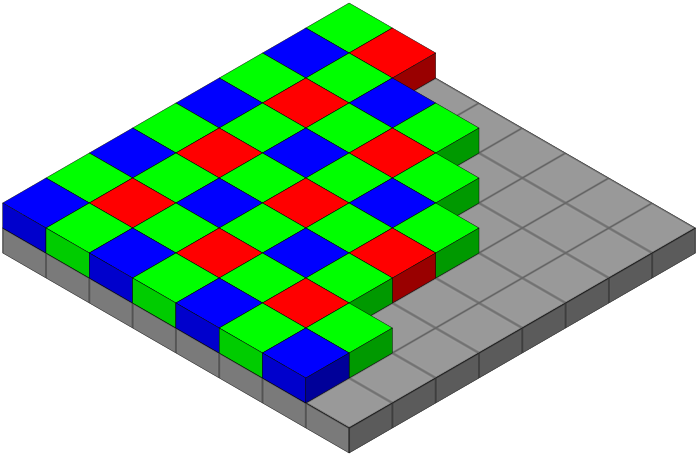
\includegraphics[width=0.5\linewidth]{figures/bayer-matrix.png} &
        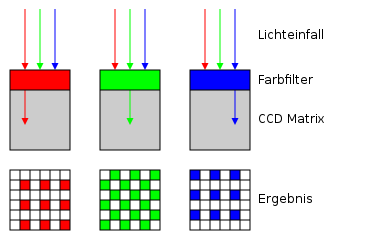
\includegraphics[width=0.5\linewidth]{figures/bayer-sensor.png}
    \end{tabular}
\end{defi}

\begin{defi}{Demosaicing}
    % TODO: https://de.wikipedia.org/wiki/Demosaicing 
    Als \emph{Demosaicing} bezeichnet man in der Digitalfotografie die Rekonstruktion einer farbigen Rastergrafik aus den Helligkeitswerten eines mit Mosaik-Farbfiltern überlagerten Bildsensors.
\end{defi}

\begin{defi}[Demosaicing]{Nearest-Neighbor}
    % TODO: https://ngi-user-guide.readthedocs.io/en/latest/demosaicing/ 
    Die \emph{Nearest-Neighbor-Methode} ist die einfachste Methode zum Demosaicing.
    Jeder interpolierte Pixel wird mit dem nächstgelegenen Pixel der gleichen Farbe gefüllt.

    \centering
    % TODO: https://wiki.apertus.org/index.php/OpenCine.Nearest_Neighbor_and_Bilinear_Interpolation
    \begin{tabular}{cc}
        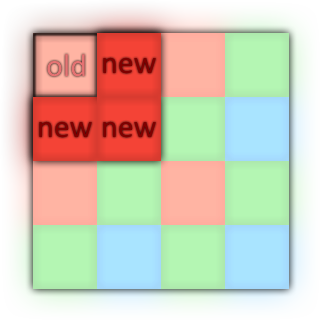
\includegraphics[width=0.15\linewidth]{figures/demosaicing-nearest-neighbour-red-blue.png} &
        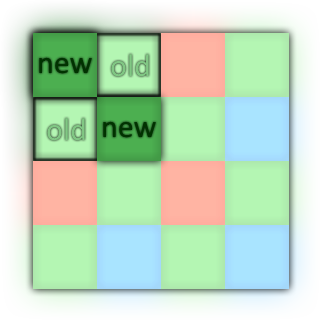
\includegraphics[width=0.15\linewidth]{figures/demosaicing-nearest-neighbour-green.png}
    \end{tabular}
\end{defi}

\begin{defi}[Demosaicing]{Bilineare Interpolation}
    Bei der \emph{Bilinearen Interpolation} werden Farbkomponenten aus den unmittelbaren Nachbarn interpoliert.

    \centering
    % TODO: https://wiki.apertus.org/index.php/OpenCine.Nearest_Neighbor_and_Bilinear_Interpolation
    \begin{tabular}{cccc}
        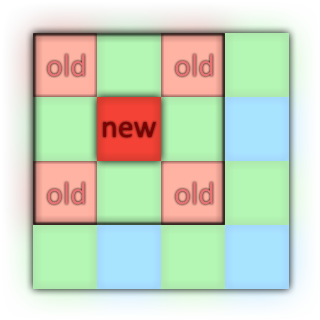
\includegraphics[width=0.15\linewidth]{figures/demosaicing-interpolation-diagonal.png}   &
        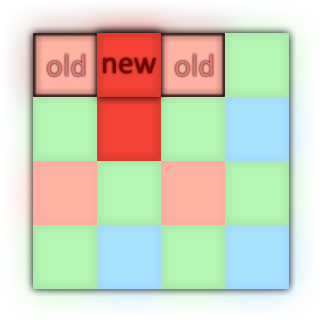
\includegraphics[width=0.15\linewidth]{figures/demosaicing-interpolation-horizontal.png} &
        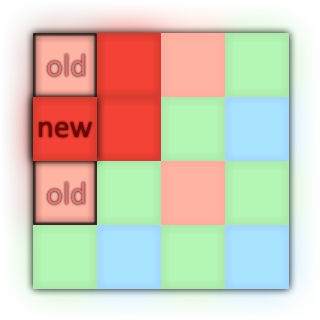
\includegraphics[width=0.15\linewidth]{figures/demosaicing-interpolation-vertical.png}   &
        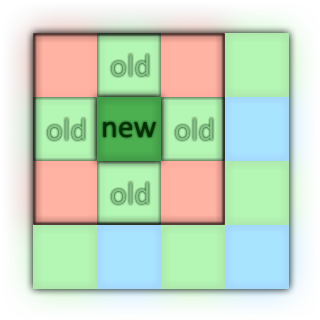
\includegraphics[width=0.15\linewidth]{figures/demosaicing-interpolation-green.png}
    \end{tabular}
\end{defi}

\begin{bonus}[Demosaicing]{Probleme}
    Bei den einfacheren Verfahren des Demosaicing kann es zu Unschärfe und anderen Bildartefakten kommen:
    \begin{itemize}
        \item \enquote{Reißverschlussartige} \emph{Schachbrettmuster} entstehen an Kanten, die nicht entlang der Farbfilter einer Grundfarbe verlaufen;
        \item \emph{Farbverschiebungen} entstehen als Alias-Effekte, wenn die Farbfiltermatrix mit regelmäßig angeordneten Bilddetails interferiert.
    \end{itemize}

    Durch Nachverarbeitung können die Ergebnisse verbessert werden.

    Auch existieren weitere Verfahren, die z. B. kanten- oder frequenzbasiert sind.

    \centering
    % TODO: https://www.semanticscholar.org/paper/Comparison-of-color-demosaicing-methods-Losson-Macaire/37df62621c6a4274e14b0ed7d01a07bc386cd37a/figure/12 
    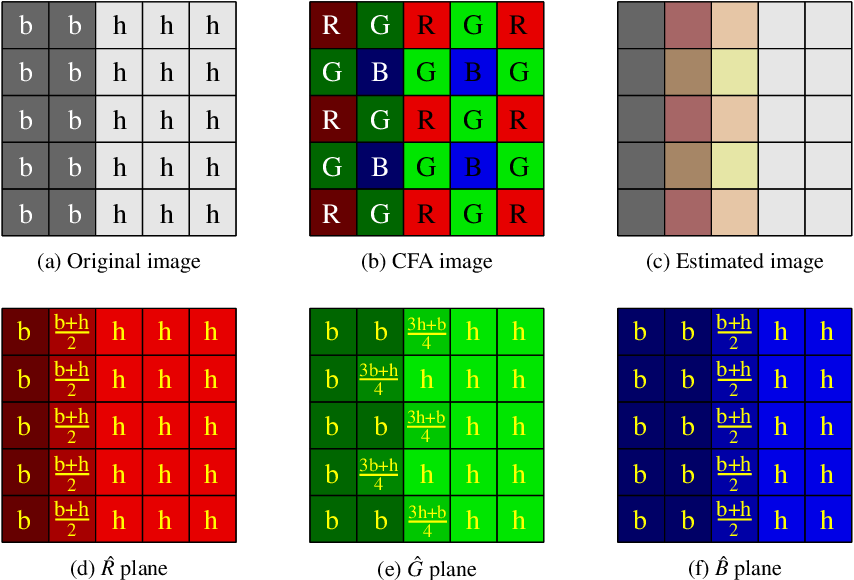
\includegraphics[width=0.75\linewidth]{figures/demosaicing-problems.png}
\end{bonus}